Chapter 2 is devoted to the theoretical part of this paper. It presents main underwater acoustics concepts, basic definitions of bubble acoustics and signal processing techniques. Also, it contains an introduction to bubble model and an explanation of the chosen approaches.

% \begin{itemize}
%     \item bubble backscattering, natural frequency, Thuraisingham and Anderson models
%     \item multiple backscattering, other models implementation
%     \item near and far field characteristics
% \end{itemize}
\section{Sound Propagation Concepts}

The sound represents the transmission of the mechanical energy that  propagates through the medium and relies on its properties \cite[p.1]{leighton_acoustic_2012}. The understanding presented below underwater acoustics basic terminology is essential for deeper comprehension of the processes that were involved in this research problem.
\subsubsection{Wavelength}
It defines the length of the wave over a unit period. It is an inverse of the wavenumber. The higher frequency, the shorter wavelength.
\begin{equation}
    \lambda = \frac{c}{f} \quad \frac{[\text{m/s}]}{[\text{1/s}]} = \text{m}
\end{equation}

\subsubsection{Speed of sound}
Generally, it is the speed of sound dependent on other parameter such as a temperature, a salinity and a depth, which make the speed of sound vary and refraction is appearing \cite[p. 28]{hodges_underwater_2011}. In order to simplify the simulation, the value of the speed of sound in a water was set at 1500 m/s. 
The equation \ref{eqn:c_water_relation} shows a relation of the speed of the sound $(c)$ to frequency $(\omega = 2\pi f)$ and a wavelength $(\lambda)$  
\begin{equation}
    c_{water} = f\lambda = \omega / k
    \label{eqn:c_water_relation}
\end{equation}
where $\omega$ is an angular frequency and $k=2\pi/\lambda$ is a wavenumber.
\subsection{Radiation of sound}

\subsubsection{Intensity} 
It is how much energy gets through the area perpendicular to the direction of the emitted wave \cite[p.18]{leighton_acoustic_2012}. The formula of acoustic intensity for a plane wave can be written in the following form:
\begin{equation}
    I = \frac{P_A^2}{2\rho c} = \frac{W}{4\pi s^2}
\end{equation}
Where $P_A$ is an acoustic pressure amplitude of the wave, $\rho$ is a density of the medium, $c$ is a speed of wave.

Where W is an energy, s is a distance from the source,
$4\pi s^2$ is a sphere surface.

\subsubsection{Intensity level}
Intensity level is a measure over some area, which is a ratio of the sound intensity $I$ to some reference intensity $I_{ref}$ \cite[p.19]{leighton_acoustic_2012}:
\begin{equation}
    IL = 10\log_{10}(\frac{I}{I_{ref}})    
\end{equation}
$I_{ref}=10^{-12}\text{W m}^{-2}$ in air.
As the pressure amplitude is proportional to the square root of intensity, we can write down sound pressure level in the form:
\begin{equation}
    SPL = 20\log_{10}(\frac{P}{P_{ref}})
\end{equation}

\subsubsection{Spherical spreading} 
The wave propagation with a $1/s^2$ dependance is defined as a spherical spreading.
% \tikz \draw (0,0) -- (2,1) -- (3,2);
% \begin{tikzpicture}
% \draw (0,0) circle (1);
% \draw (0,0) circle (1.5in);
% \end{tikzpicture}
\subsubsection{Attenuation  of sound}
The process of absorbtion and scattering of the sound can be defined as an attenuation. 

It is an amount of the transmitted sound signal received back by a receiver.

\subsubsection{Scattering cross-section} 

The amount of energy transmitted sound wave being reflected by the small object in the direction of the receiving system is evaluated with a scattering cross-section, the ratio of the total scattered power from the object to incident plane wave intencity \cite[p. 40]{hodges_underwater_2011}:
\begin{equation}
    \sigma_{bs}=\frac{W}{I_{inc}}
\end{equation}
We often want to determine exactly how much of an incident acoustic beam's energy is scattered by a bubble, rather than being lost through thermal and viscous dissipation.

\section{Signal Processing Concepts}
% \begin{itemize}
    %     \item reconstruction of the bubble frequency response from the received signal
    %     \item beamforming
    %     \item cross-correlation, matched filtering
    %     \item sonar equation
    % \end{itemize}
    
\subsection{Beamforming}

A beamforming is a way of processing the received or transmitted signal, so that we can direct the directed and amplified signal from teh projector with multiple receivers or transmitters, therefore improving the SNR and eliminating unwanted interfering signals. Also, it can be referred as a spatial filtering.

Withing the scope of the work we have used beamforming in the sonar environment. A conventional beamformer in the form of the delay-and-sum was used. 

\subsection{SONAR}

\subsubsection{SIMO-sonar}

The general principle of the projector SIMO-sonar is in the following way:  the signal is emitted with a single transducer and receiving a signal back with several receivers, which in our case were hydrophones. Also, it can be considered with another interpretation. For example, we provide a single output, and obtain multiple input data.
    
The sonar type is the SIMO-sonar, as we needed to start with a simple model of the current research. The experiments with a MIMO-sonar can be implemented for further research therefore expanding the complexity and variability of usages of the developed model, as [this type provides an improved resolution and enhances the signal-to-noise ratio of the received signal] (http://jset.sasapublications.com/wp-content/uploads/2017/09/6702529.pdf).
    
	
\subsection{Sonar Equation }
The Sonar equation is a fundamental tool in underwater acoustics used to predict the performance of sonar systems. 
The basic form of the Sonar equation is:
\begin{equation}
    SNR=SL-TL+TS-NL
\end{equation}

Where
SNR is the signal-to-noise ratio,
SL is the source level,
TL is the transmission loss,
TS is the target strength, and
NL is the noise level.

To implement the Sonar equation, one needs to calculate or estimate each of these parameters. 
Source level (SL) represents the acoustic power radiated by the sonar system, which can be determined based on the characteristics of the sonar transducer and the electrical input power. 
Transmission loss (TL) accounts for the attenuation of sound energy as it propagates through the water, considering factors such as spreading loss, absorption, and bottom and surface reflections. 
Target strength (TS) quantifies the amount of sound energy reflected or scattered by the target, which depends on its size, shape, and composition. 
Noise level (NL) encompasses all sources of ambient noise in the environment, including thermal noise, wind-generated noise, biological noise, and anthropogenic noise.


\subsubsection{Near- and far-field}
The phase difference that comes from the path difference is proportional to the ration of the path to the wavelength \cite[p.30]{leighton_acoustic_2012}.

\[D_\text{Near to far field} = L_s^2/\lambda\] 
where $L_s$ is the spacing between receivers
% find an image of hydrophones lobes with near and far field comparison

\section{Bubble models}
Bubble's acoustic frequency response can depend on multiple factors. Among them are a bubble radius, water pressure, ensonification frequency.

For the simplicity, in most studies the bubble shape is assumed to be spherical, as the optical equipment at long distances can't provide an accurate estimation of the bubble's shape and size \cite[p.2]{zhang_efficient_2022}. 

\textbf{Bubble flare} A continuous column of bubbles with the different radii which is emitted with a bubble generator. Minimum bubble size that the machine could produce were 

\subsubsection{Resonance frequency}
Due to the mass-spring system which appears from the interaction of the incoming wave with a bubble. The gas inside and the surface tension in the bubble with the liquid   


\subsubsection{Target strength} 
It is the measure of the single object's (e.g. bubble) reflection of the transmitted signal. %my words , find justification
% bubble backscattering, natural frequency, Thuraisingham and Anderson models
\subsection{Single bubble model}

Single bubbles can be used as comparison to the fish in the water as they have bludders filled with an air, and this is usually a typical reflective surface recorded with a sonar.

\begin{itemize}
    \item Anderson
    Anderson model provides a modal solution and allows to model the backscattering cross-section of a single bubble for $ka > 1$ \cite{anderson_sound_2005}.

    \item Thuraisingham

    In this paper of Zhang et al. 2022 \cite{zhang_efficient_2022} modal solution is used when ka > 1, and Thuraisingham solution is preferred for the ka<1, as the first doesn't consider the bubble damping effect.  Such approach can be used for our multiple compund bubble simulation.

    \item Church, Medwin,

    Andreeva is for fish.

\end{itemize}

% There is a general formula of the gas bubble's rising velocity based on the bubble's volume, which allows us not to consider the bubble shape and its change during the rising process????(whose citation)
\subsubsection{Anderson model}
The process of establishing the model for the acoustic frequency response of the bubble dates back to the paper of Anderson in 1950 \cite{anderson_sound_2005}. Initially, the theory of Rayleigh scattering has provided a big input into the scatterers which are comparable to a wavelength. While this work presented spheres with medium-like acoustic properties, and dimensions are as a couple  wavelengths. Using provided calculation we can obtain the pressure and the total energy in the scattered wave.

The following limitation of this model which should be considered is when ka approaches 0. That which means that the radius of sphere becomes less than a wavelength. For the cases when ka <1 or >1 there are no limitations.

This paper results can be used for comparison with other models available nowadays. The implementation in Matlab has allowed us to see how the peak at resonance frequency corresponds to the one of Thuraisingham model. However, at higher frequencies we can observes additional peaks, which indicate other modes of the fluid sphere, when $ka$ is closer or over 1.
% We can express cross-section scattering using a relation of the reflectivity and a measure of the amount of power scatterer diverting from the original wave. That allows to obtain the total 

\subsubsection{Thuraisingham model}
The scattering cross-section $\sigma_s$ of a single bubble is a ratio of the energy loss averaged over time while being scattered from the bubble to the intensity of incident signal \cite[p.408]{thuraisingham_new_1997}. Thuraisingham formula for the scattering cross-section with the condition of a spherical pulsation of the bubble was presented in this form: 

\begin{equation}\label{eq:thuraisingham}
    \sigma_s=\frac{4\pi a^2}{\delta^2 + (\frac{\omega_r^2}{\omega^2}-1)^2}\frac{(\frac{\sin ka}{ka})^2}{1+(ka)^2}
\end{equation}
Where $a$ is a bubble radius, $k$ is a wavenumber in the water, $\delta$ is a damping constant ,$\omega_r$  is the resonance frequency, $\omega$  is the angular frequency.

This model applies over all values of $ka$. After that a model was optimised by Li et al. \cite[]{li_broadband_2020} for the omnidirectional breathing mode. As the impact of the last factor decreases with the increase of the $ka$-value, we require more adaptable model to different modes. In this paper Li et al. have used for $ka << 1$ a Thuraisingham formula and for $ka>1$ was used an adjusted modal solution.

% my plots are better to be placed to the section of "my simulations". Here I propose to insert pictures from papers/books
\begin{figure}[H]
    \centering
    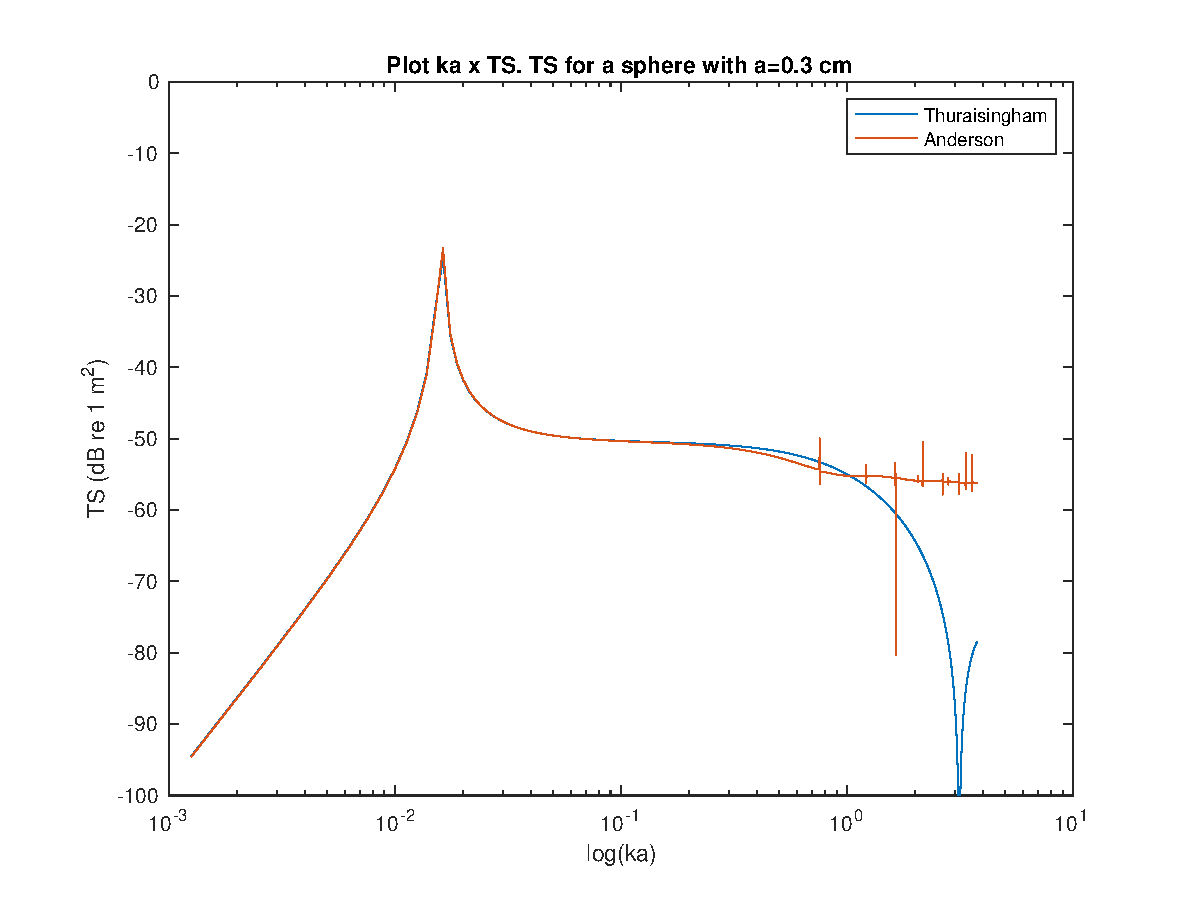
\includegraphics[width=0.7\textwidth]{thur-and-models.eps}
    \caption*{Target strength over $ka$-values for a Thuraisingham and Anderson solutions of a single bubble of radius a = 0.3 cm}
    \label{fig:thur-anderson}
\end{figure}

Figure \ref*{fig:thur-anderson} shows a plot of the single bubble target strength against  $ka << 1$, and significantly larger values $ka > 1$. The highes peak corresponds to the resonance frequency of the bubble, following smaller peaks of the modal solution might correspond to the normal modes of the bubble, which occur as a resulting oscillations. Yet it doesn't take into account the damping effect present in a bubble.


\subsection{Multiple bubble model}

For more than one bubble we can add various scenarious for bubbles' location in space, distance between each other, their dimensions, dynamics, and interactions. Those new properties pose more challenges in constructing a valid model for multiple bubbles.

Among the possible real-world applications are gas seapages underwater, bubble curtains which play role of sound attenuators.

% math assumptions and formulations

\subsubsection{Volume-scattering strength} 
In case we have more than one bubble, where we were describing it with a target strength, the volume backscattering strength should be used instead.
\[s_v = \int\sigma_{bs}n(a)\]
\[S_v = 10\log_{10}(s_v)(dB\;re\;1m^2)\]

% More bubbles are added

\subsection{Multiple scattering }

Leblond et al. paper states that for multiple discrete bubbles, we can neglect the effect of the multiple scattering \cite[]{leblond_acoustic_2014}. 
\textcolor{red}{Foldy paper equation explanation and concept of the multiple scattering}

When the signal is emitted, the scatterer removes from the wave a specific amount of flux which is equal to the its extintion cross section multiplied by flux per unit area. This amount is partially absorbed and scattered. The next step lies in adding up all the scattering from the received transmitted signal scatterer to other bubbles, then repeating the procedure in the regard of other bubbles, till all scatterers in the close enough vicinity of each other got an interaction with each other.

\begin{figure}[H]
    \centering
    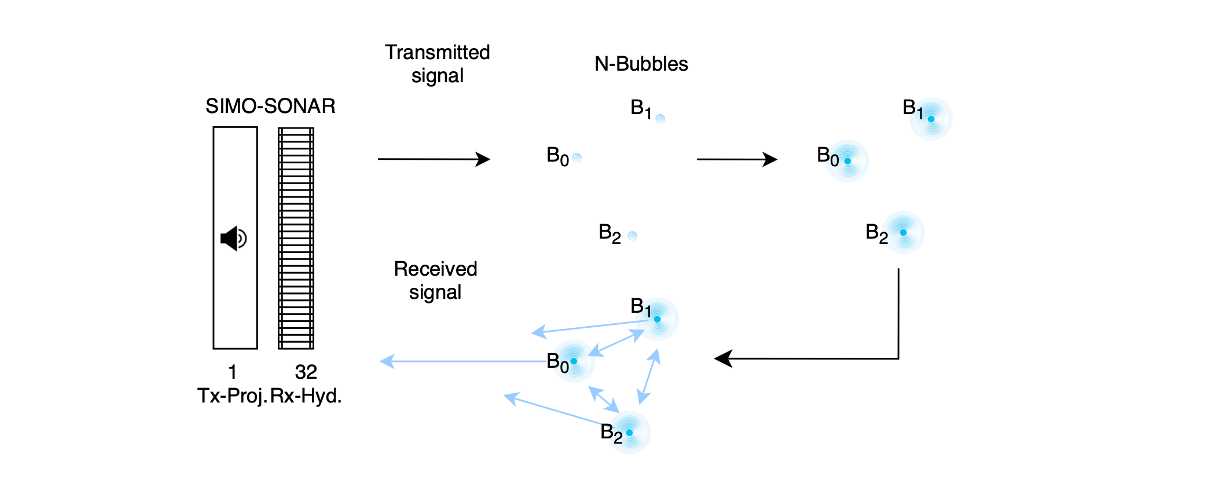
\includegraphics[width=0.7\textwidth]{multiple-scattering.png}
    \caption*{The scheme of the multiple scattering}
    \label{fig:multiple-scattering}
\end{figure}

But this concept is applicable when amount of scatterers is sufficiently small, otherwise they start interacting with each other and no longer act as a scatter independently. %source????? Foldy or Hazard?

Hazard and Cassier paper provides a mathematical point of view at the multiple scattering with a justification of the Foldy-Lax model. This model help to get an approximation of scattered waves in a deterministic as well as in a random media. Also, local error estimates for circular objects in 2D problem were obtained in the scope of results of this paper.

- Foldy, Leslie L. ‘The Multiple Scattering of Waves. I. General Theory of Isotropic Scattering by Randomly Distributed Scatterers’. Physical Review 67, no. 3–4 (1 February 1945): 107–19. https://doi.org/10.1103/PhysRev.67.107.

- Multiple Scattering of Acoustic Waves by Small Sound-Soft Obstacles in Two Dimensions: Mathematical Justification of the Foldy–Lax Model, Hazard and Cassier

\section{Reconstruction of the bubble frequency response}

It will allow demonstrating the ability to invert the model to find individual bubble contributions from compund analysis.
The following equation\ref{eqn:reconstruction_bubble} was the base of the calculations:

\begin{equation}\label{eqn:reconstruction_bubble}
    R = T \times H + N
\end{equation}
where R is a received signal, T is a transmitted signal by sonar, H is frequency response of the bubble, N is an added background noise.
